\documentclass[11pt]{article}

\usepackage[margin=1in]{geometry}
\usepackage[utf8]{inputenc}
\IfFileExists{lmodern.sty}{\usepackage[T1]{fontenc}\usepackage{lmodern}}{}
\usepackage{microtype}
\usepackage{amsmath,amssymb}
\usepackage{booktabs}
\usepackage{tabularx}
\usepackage{enumitem}
\usepackage{listings}
\usepackage{xcolor}
\usepackage{tikz}
\usetikzlibrary{positioning,arrows.meta,fit,backgrounds}
\usepackage[hidelinks]{hyperref}

\lstset{
  basicstyle=\ttfamily\small,
  columns=fullflexible,
  keepspaces=true,
  frame=single,
  framerule=0.3pt,
  rulecolor=\color{black!30},
  xleftmargin=0.5em,
  xrightmargin=0.5em,
  commentstyle=\color{black!55},
  morecomment=[l]{--},
  literate={<=}{{$\le$}}1
}

\newcommand{\Shat}{\hat{S}}
\newcommand{\SE}{\mathrm{SE}}
\newcommand{\E}{\mathbb{E}}

\title{Auditable Search for Agentic Quant Research\\[0.3em]\large Draft white paper}
\author{Kevin Lei}
\date{October 18, 2026}

\begin{document}
\maketitle

\begin{abstract}
Frontier LLM agents can search large hypothesis spaces cheaply, and in mathematics that search yields results because a formal checker rejects every candidate that does not follow from the stated definitions. This paper proposes a design for retail quantitative research that borrows the structure but not the certainty: agents generate trading hypotheses freely, and a small controlled kernel enforces specific program-level invariants and keeps a complete, auditable record of what every agent saw. The kernel has two parts. A typed strategy language and a controlled evaluator enforce specified constraints on data availability, order timing, and unit consistency, while separate execution models estimate whether trades could plausibly have filled. An experiment ledger records every evaluation and every result disclosed to an agent, so that multiplicity can be estimated and the whole adaptive search procedure can be tested on simulated markets with no edge. Formal methods can make certain errors impossible; they cannot turn noisy historical evidence into a correctness certificate. Whether the full system actually controls false discoveries is a claim to be demonstrated by null simulation, not assumed. We identify small-capacity strategies, venue structure on Hyperliquid, and slowly digested information as plausible research directions for retail, pending point-in-time feasibility checks.
\end{abstract}

\section{Motivation}

Agentic mathematics works as a search problem with a learned heuristic. Many subagents propose candidate lemmas, proof steps, or constructions at high throughput. The LLM acts like the heuristic in classical tree search (GOFAI-style best-first search, or MCTS in AlphaGo-like systems): it decides which branches look promising, not which are correct.

Correctness comes from somewhere else. A proof assistant such as Lean has a small trusted kernel that checks whether each candidate proof follows from the formal definitions, cheaply and mechanically. Because wrong guesses cost almost nothing, the heuristic is allowed to be wild. The kernel's guarantee is also narrower than it looks: it certifies that a proof matches the formal statement, not that the formal statement captures the intended question. A trading evaluator has the same weakness in a stronger form, since it can compute a perfectly correct result for an incorrectly modeled market.

The question for retail traders is how much of this structure carries over to strategy research, with agents as tireless research assistants and formal constraints as part of the kernel. Retail cannot match institutional data, latency, or headcount, but agents lower the cost of research labor. Many current agentic trading tools focus on order entry through a chat interface; this paper is about automating and auditing the research loop instead. Whether agents generate better hypotheses than simpler search methods is itself an open empirical question that the roadmap tests directly.

\section{The core obstacle: a noisy, exploitable verifier}

The analogy to mathematics breaks at the verifier. A proof checker is exact and cannot be fooled. A backtest is a noisy estimate on non-stationary data, and searching harder against it produces better-looking results whether or not any edge exists.

A pass/fail filter does not avoid this. Accepting only strategies above a Sharpe threshold is still selection, and selection over many candidates behaves like optimization. The example below is illustrative: it assumes independent, stationary, roughly Gaussian returns and independent trials, all of which real Hyperliquid strategies violate to some degree. Under those assumptions, over $T$ years of data the standard error of an annualized Sharpe estimate is approximately
\begin{equation}
  \SE(\Shat) \approx \frac{1}{\sqrt{T}}.
\end{equation}
With 5 years of data, that is $1/\sqrt{5} \approx 0.45$. Suppose the swarm tests 1{,}000 strategies with zero true edge and keeps any with an estimated Sharpe above 1, a threshold $\sqrt{5} \approx 2.24$ standard errors above zero:
\begin{equation}
  P(\Shat > 1 \mid S = 0) = 1 - \Phi(\sqrt{5}) \approx 1.27\%.
\end{equation}
About 13 null strategies pass. Add 10 genuine strategies with true Sharpe $0.5$; each passes with probability $1 - \Phi(0.5\sqrt{5}) \approx 13\%$, so roughly 1.3 survive. The accepted set is about 90\% false discoveries, even though each individual test looked reasonable.

More generally, the expected best of $N$ null strategies is the standard error times the expected maximum of $N$ standard normals, which grows like $\sqrt{2\ln N}$ to leading order:
\begin{equation}
  \E\Big[\max_{i \le N} \Shat_i\Big] = \SE \cdot \E\Big[\max_{i \le N} Z_i\Big],
  \qquad
  \E\Big[\max_{i \le N} Z_i\Big] \approx \sqrt{2 \ln N}.
\end{equation}
For $N = 1{,}000$, the leading-order formula gives $0.45 \times 3.72 \approx 1.66$. The exact expected maximum of 1{,}000 standard normals is about $3.24$, which gives $1.45$. Either way, the luckiest noise looks like a strong strategy. Agents make this worse in three ways:
\begin{enumerate}
  \item \textbf{Hidden trials.} An agent that tweaks a parameter, looks at the result, and tweaks again has run many tests while submitting one.
  \item \textbf{Unclear effective $N$.} A thousand near-duplicates are neither 1{,}000 independent tests nor one.
  \item \textbf{Non-stationarity.} Even a correctly validated edge only shows the edge existed in the sample period.
\end{enumerate}
The design goal follows: the system must make the complete history of what agents saw and decided auditable, so that the selection procedure can be evaluated as a whole rather than one test at a time.

\section{Architecture: a small trusted kernel}

The system splits into an untrusted generator and a trusted kernel, and the only way to obtain a backtest result is through the kernel (Figure~\ref{fig:arch}).

\begin{figure}[ht]
\centering
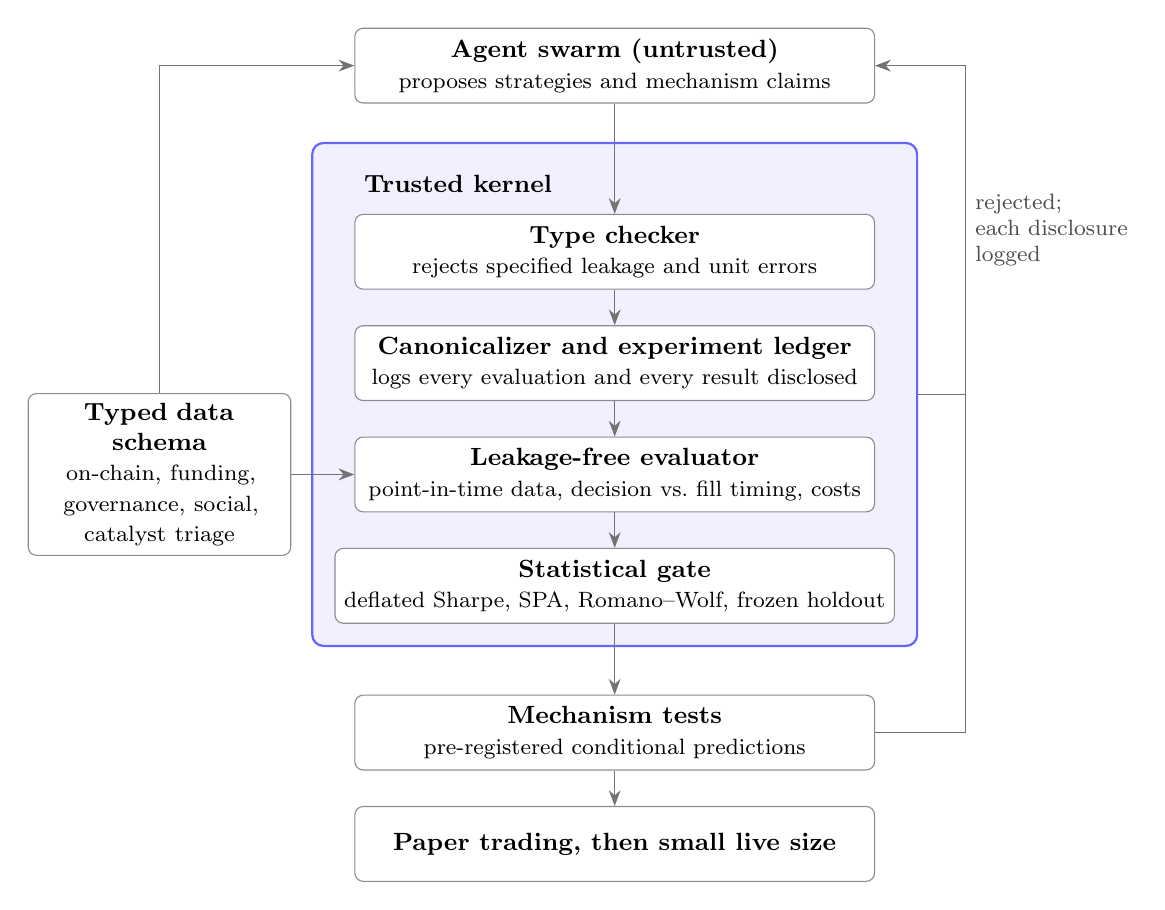
\begin{tikzpicture}[
  font=\small,
  node distance=0.45cm,
  stage/.style={draw=black!45, rounded corners=3pt, align=center, minimum width=6.6cm, minimum height=0.95cm, fill=white},
  side/.style={draw=black!45, rounded corners=3pt, align=center, text width=3.1cm, minimum height=1.6cm},
  arr/.style={-{Stealth[length=2mm]}, draw=black!55}
]
  \node[stage] (agents) {\textbf{Agent swarm (untrusted)}\\ \footnotesize proposes strategies and mechanism claims};
  \node[stage, below=1.4cm of agents] (tc) {\textbf{Type checker}\\ \footnotesize rejects specified leakage and unit errors};
  \node[stage, below=of tc] (ledger) {\textbf{Canonicalizer and experiment ledger}\\ \footnotesize logs every evaluation and every result disclosed};
  \node[stage, below=of ledger] (eval) {\textbf{Leakage-free evaluator}\\ \footnotesize point-in-time data, decision vs.\ fill timing, costs};
  \node[stage, below=of eval] (gate) {\textbf{Statistical gate}\\ \footnotesize deflated Sharpe, SPA, Romano--Wolf, frozen holdout};
  \node[stage, below=0.9cm of gate] (mech) {\textbf{Mechanism tests}\\ \footnotesize pre-registered conditional predictions};
  \node[stage, below=of mech] (paper) {\textbf{Paper trading, then small live size}};
  \node[font=\small\bfseries, anchor=south west] (ktitle) at ([yshift=0.15cm]tc.north west) {Trusted kernel};
  \node[side, left=0.8cm of eval] (data) {\textbf{Typed data schema}\\ \footnotesize on-chain, funding, governance, social, catalyst triage};

  \begin{scope}[on background layer]
    \node[draw=blue!60, thick, rounded corners=4pt, fill=blue!6, inner sep=8pt, fit=(tc)(gate)(ktitle)] (kernel) {};
  \end{scope}

  \draw[arr] (agents) -- (tc);
  \draw[arr] (tc) -- (ledger);
  \draw[arr] (ledger) -- (eval);
  \draw[arr] (eval) -- (gate);
  \draw[arr] (gate) -- (mech);
  \draw[arr] (mech) -- (paper);
  \draw[arr] (data) -- (eval);
  \draw[arr] (data.north) |- (agents.west);
  \draw[arr] (kernel.east) -- ++(0.6,0) |- (agents.east)
    node[pos=0.25, right, align=left, font=\footnotesize, text=black!70] {rejected;\\each disclosure\\logged};
  \draw[draw=black!55] (mech.east) -| ([xshift=0.6cm]kernel.east);
\end{tikzpicture}
\caption{Agents propose freely; results come only through the kernel.}
\label{fig:arch}
\end{figure}

Agents propose strategies with mechanism claims; the kernel type-checks, canonicalizes and logs, evaluates, and gates them. Every result shown to an agent, including for rejected candidates, is recorded in the ledger, because it can shape what the agent tries next.

The kernel's source code should be small, but the trusted computing base is larger than the kernel. Its correctness also depends on:
\begin{itemize}
  \item historical data reconstruction and ingestion, including revisions and timestamps;
  \item the DSL compiler and runtime;
  \item the market simulator, fee model, and execution model;
  \item the statistical implementations and the ledger's storage.
\end{itemize}
Each of these needs stated invariants and tests. ``Results come only through the kernel'' is a deployment requirement, not a property of the design: agents must run in an environment with no direct access to market data or arbitrary compute over it. An agent that can load a CSV and run its own backtest can do unlogged research, and nothing in the kernel would know.

\section{A typed strategy language}

Agents do not write arbitrary Python backtests. They write strategies in a small domain-specific language designed to rule out specified classes of research bugs before anything runs. The properties below are design targets; each must be stated as a formal invariant and tested, including against strategies written specifically to evade it.

\paragraph{Causality in data and in execution.} A strategy is a causal stream transformer, formally a Mealy machine: its output at time $t$ depends only on inputs it has received. That alone is not enough. A type signature only describes an interface; the guarantee comes from the runtime feeding the machine only point-in-time data and enforcing four distinct times: when data became available, when the strategy decided, when its order could be submitted, and when that order could actually fill. A strategy that reads a candle's close at 12:00 and fills at that close is causal in its inputs but still leaks through execution. The runtime can enforce that these times are ordered and that an order's fill conditions were met in the recorded book. It cannot establish that a fill would really have happened: queue position, cancellations, competing orders, and latency are not fully visible in historical data, so fills are an estimate from a calibrated execution model. Event-driven engines such as QuantConnect's LEAN already separate a time frontier from fill models, and the DSL should at least match that.

\begin{lstlisting}
-- A strategy consumes point-in-time observations and emits orders
type Strategy = Mealy (Obs Event) Order

-- Each observation records when it became knowable and which revision it is
data Obs a = Obs { eventTime :: Time, knownAt :: Time, revision :: Int, value :: a }

-- The simulator, not the strategy, decides submission and fill times
data Fill = Fill { decidedAt :: Time, submittedAt :: Time
                 , filledAt :: Time, price :: Price }
\end{lstlisting}

The evaluator, not these types, enforces the runtime invariant
\begin{equation}
  t_{\mathrm{known}} \le t_{\mathrm{decision}} \le t_{\mathrm{submission}} \le t_{\mathrm{fill}}
\end{equation}
for every input to a decision, together with the requirement that the order's fill conditions hold in the recorded book at $t_{\mathrm{fill}}$.

\paragraph{Units, dimensions, and time bases.} Prices, sizes, funding rates, and volatilities carry types, so adding a price to a funding rate fails to compile. Rates also carry their time basis: an hourly and an annualized funding rate are both dimensionless ratios, but combining them without an explicit conversion is a type error. Normalized features get their own dimensionless type. Types do not stop a feature from being normalized with future data; that is the runtime's job.

\paragraph{Composition.} Causal transformers compose: features feed signals, signals feed sizing, sizing feeds risk limits. With objects, morphisms, and parallel composition specified precisely, this should form a symmetric monoidal category, which would give the canonicalizer in Section~\ref{sec:ledger} algebraic laws to rewrite with. That structure is a construction to carry out, not yet a result, and each rewrite law must be shown to preserve full trading semantics, including state, order timing, fees, and floating-point behavior.

\paragraph{Execution realism.} Fees, funding payments, slippage, and latency are part of the evaluator's semantics rather than optional parameters. On Hyperliquid this means modeling the fee tier a small account actually pays, funding schedules, and order-book depth at the decision time. These models are only as good as their calibration, so the paper treats them as validated components with stated error bounds, not as solved.

\section{Canonicalization and the experiment ledger}\label{sec:ledger}

The ledger makes the research process auditable; it does not by itself produce a trial count that can be plugged into a correction. A canonical strategy is a program, while a statistical trial is about information: what an agent saw and how that shaped what it selected next. An agent that inspects one strategy's drawdown, yearly returns, and cost sensitivity, then proposes something new, has spent multiplicity without creating any new canonical form. Conversely, rerunning an identical deterministic backtest, or rejecting a strategy at the type checker before it touches data, spends none.

\paragraph{What the ledger records.} Four things, kept distinct:
\begin{enumerate}
  \item \textbf{Strategy identity:} the canonical form, so equivalent programs are recognized.
  \item \textbf{Experiment identity:} strategy, parameters, asset universe, data window, dataset version, availability-time conventions, execution and fee model versions, simulator version, and random seeds.
  \item \textbf{Disclosures:} every statistic or plot returned to an agent, including for rejected candidates.
  \item \textbf{Selection decisions:} which candidates an agent or the gate chose to pursue, and what it had seen at that point.
\end{enumerate}
Multiplicity is then estimated from this history, and those estimates are checked by testing the whole procedure on null markets (Section~\ref{sec:roadmap}).

\paragraph{Canonical forms.} Strategies are rewritten using the DSL's algebraic laws, for example commuting independent features or folding constant transforms. Equality saturation with e-graphs, as in the egg library, is a practical tool for this, with an important limit: it finds expressions provably equal under the supplied rewrite rules and extracts one by a cost model. It does not produce a unique canonical form for every semantically equivalent program, and results depend on rule coverage and resource limits. The claim is therefore narrower: the system detects some provable equivalences, conditional on the soundness of its rewrite rules.

\paragraph{Effective $N$.} Strategies that differ syntactically can still behave almost identically. Clustering return streams by correlation gives one estimate of the effective number of independent trials, in the spirit of Bailey and L\'opez de Prado, but it is a heuristic. The correct adjustment depends on the joint distribution of the test statistics, and the correlations are estimated on the same sample being searched. The gate therefore reports how its decisions change across several effective-$N$ estimates, and treats a promotion that holds only under the most favorable estimate as fragile.

\paragraph{Search guidance.} Agents can query which regions of strategy space are already explored, steering generation toward novel hypotheses. This is itself a feedback channel: telling agents where past results were good or bad is a disclosure, and it is logged and accounted for like any other.

\section{The statistical gate}\label{sec:gate}

Individually valid tests do not make a valid combined procedure, so each search campaign runs a fixed gate written down before the campaign starts. Its error rates are claimed only as far as the simulations in Section~\ref{sec:roadmap} confirm them, and only for the market models simulated.
\begin{enumerate}
  \item \textbf{Search period only.} Agents see results from a research period. The holdout period is never shown to them.
  \item \textbf{Screen.} Candidates must pass a deflated Sharpe threshold computed at each of several effective-$N$ estimates, using the largest. That is conservative only relative to the estimators chosen, not a guaranteed bound.
  \item \textbf{Global test.} Hansen's SPA runs over every strategy evaluated in the campaign and asks whether any beats the benchmark. If it does not reject, the campaign promotes nothing. Because the family was generated adaptively, its stated error rate is approximate.
  \item \textbf{Individual decisions.} Romano--Wolf stepdown on the screened candidates gives per-strategy adjusted $p$-values with family-wise error control. SPA answers whether anything works; Romano--Wolf answers which candidates to keep.
  \item \textbf{Mechanism check.} A candidate whose pre-registered mechanism prediction fails is removed from the finalists. There is no override by a higher statistical threshold.
  \item \textbf{Freeze.} The finalists, the promotion rule, and the multiple-comparison correction across finalists are fixed before the holdout is opened.
  \item \textbf{Holdout batch.} All finalists are evaluated together, once. A finalist is promoted to paper trading only if its net-of-cost holdout return is positive and its holdout Sharpe passes a preset significance level after Holm correction across finalists. The thresholds are parameters; the structure is fixed.
  \item \textbf{No recycling.} A strategy modified after its holdout result cannot be retested on that holdout. A holdout used by one campaign is spent: the next campaign evaluates on a later period, and the old holdout becomes part of its search data.
\end{enumerate}

\begin{table}[ht]
\centering
\small
\begin{tabularx}{\textwidth}{@{}>{\raggedright\arraybackslash}p{3.3cm}>{\raggedright\arraybackslash}X>{\raggedright\arraybackslash}X@{}}
\toprule
Method & What it controls & Key assumption to check \\
\midrule
Deflated Sharpe ratio & Selection bias from $N$ trials, non-normal returns, track length & A valid effective $N$ and the Sharpe sampling model \\
White's Reality Check, Hansen's SPA & Whether the best of a family beats a benchmark & A correctly specified family and a suitable bootstrap for dependent data \\
Romano--Wolf stepdown & Family-wise error across correlated strategies & Resampling assumptions; it controls error, it does not certify survivors \\
Benjamini--Hochberg & False discovery rate & Valid $p$-values and acceptable dependence \\
Probability of backtest overfitting (CSCV) & Instability of the in-sample selection procedure & A diagnostic of the procedure, not a forecast of future profit \\
\bottomrule
\end{tabularx}
\caption{Statistical methods used by or available to the gate.}
\end{table}

The deflated Sharpe ratio compares the observed Sharpe with the Sharpe expected from the best of $N$ null trials, adjusting for skewness, kurtosis, and sample length. Unlike Section~2, it works in per-period units:
\begin{equation}
  \mathrm{DSR} = \Phi\!\left( \frac{(\Shat - S_0)\sqrt{T-1}}{\sqrt{1 - \hat{\gamma}_3 \Shat + \frac{\hat{\gamma}_4 - 1}{4}\Shat^2}} \right).
\end{equation}
Here $T$ is the number of return observations, $\Shat$ is the Sharpe per observation period (for daily data, roughly the annualized Sharpe divided by $\sqrt{252}$, or $\sqrt{365}$ for markets that trade every day), and $S_0$ is the expected maximum per-period Sharpe under the null given $N$ effective trials. $\hat{\gamma}_3$ is skewness and $\hat{\gamma}_4$ is ordinary kurtosis, which equals 3 for a normal distribution, not excess kurtosis. The formula assumes independent, identically distributed observations. Autocorrelation changes the Sharpe ratio's sampling distribution \cite{lo2002}, and swapping in a robust variance does not by itself fix the null distribution of the maximum across correlated strategies. The DSR expression is therefore a baseline under its stated assumptions; the gate's actual thresholds are calibrated with time-series resampling, such as a block bootstrap, and with the simulations in Section~\ref{sec:roadmap}. Folds use walk-forward splits with purging at boundaries so overlapping labels do not leak.

\paragraph{The holdout.} Every query to a holdout leaks some information, and what matters is how much each answer reveals, not just how many queries there are. The reusable holdout of Dwork et al.\ (Thresholdout) releases holdout answers through a noisy threshold mechanism and gives formal guarantees under adaptive queries. If Thresholdout is not implemented, the system's hard query budget is a heuristic safeguard only, and the paper does not claim formal adaptive validity for it.

\section{Mechanism obligations}

Every strategy must ship with a stated mechanism, and the mechanism must imply tests beyond PnL. These tests are additional empirical checks that can count against a strategy; they are not a second verifier comparable to a proof checker. The obligation has three parts:
\begin{enumerate}
  \item \textbf{Counterparty.} Who is on the other side of the trade, and why are they willing to trade at this price? The counterparty need not be wrong: forced sellers at liquidation, hedgers paying for immediacy, and traders reducing inventory can all be acting rationally.
  \item \textbf{Conditional predictions.} If the mechanism is real, the effect should vary in specified ways, with stated tolerances. A liquidation-cascade strategy should earn more when positions are crowded near liquidation and less when funding has normalized. A slow-information strategy should decay as the information ages.
  \item \textbf{Capacity and decay.} Roughly how much size the effect supports, and what would make it disappear.
\end{enumerate}
Conditional predictions are written down before they are tested and logged in the ledger like any other experiment. Ideally they are tested on data not used to find the strategy, since predictions checked on the same sample are not independent of the PnL result. A failed prediction is evidence that the stated explanation is wrong, not proof that the strategy is: it may work for another reason, or the test may lack power. Under the gate in Section~\ref{sec:gate}, a failed pre-registered prediction removes the candidate from that campaign's finalists; it can be re-proposed with a revised mechanism in a later campaign, evaluated on fresh data.

A working hypothesis of this design is that LLMs are most useful here for proposing economically plausible ideas rather than for blind search. That hypothesis should be tested against simpler generators, such as random or genetic search over the same DSL, using the same gate.

\section{Integrating disparate data}

Category theory offers a principled way to state how data from different sources fits together. It enforces consistency with the mappings you declare; it cannot tell you whether those mappings match reality. Every new source also multiplies the space of possible strategies, so integration and multiplicity accounting have to be designed together.

\paragraph{Schemas as categories.} In Spivak's framework, a database schema is a category and an instance is a set-valued functor on it. Objects are entity types such as Token, Wallet, Proposal, and Post; morphisms are functional relationships. Many-to-many, time-varying relationships need their own entities: a wallet does not map to one token, so the schema has a Position object with morphisms to Wallet, Token, and an interval of validity. Ologs are the human-readable version of the same idea.

\paragraph{Migration as functors.} Functorial data migration, implemented in the CQL tool, moves data between schemas along functors and preserves the declared relationships. It does not solve entity resolution: if two sources use different identifiers for the same token, or the same identifier for different contracts, a migration can be formally correct and still wrong. Entity matching needs its own tests. An open design question is whether this framework earns its complexity over a carefully typed, versioned relational schema; its main advantage would be that migrations and their consistency properties are explicit and checkable.

\paragraph{Point-in-time data.} A \texttt{knownAt} field is necessary but not sufficient. Real data is revised, backfilled, delayed by ingestion, and sometimes mistimestamped. The store keeps immutable revisions with lineage, so a query ``as of time $t$'' returns what was actually available then. A derived observation is available no earlier than the latest of its inputs, which is a necessary condition for correctness, not a complete one.

\paragraph{Cross-source hypotheses.} Agents can propose strategies as paths through the schema, for example from a governance proposal, to the token it affects, to the wallets most exposed to that token, to their liquidation levels. Each such path is a hypothesis, and each is recorded in the ledger. A schema with many sources makes it easy to generate many plausible-sounding paths, which is exactly why the gate must see all of them.

\section{Research directions for retail edge}

The method is not the edge: institutions already run automated alpha research. The directions below are hypotheses about where a small account might compete, not demonstrated sources of return, and each depends on the data actually supporting a point-in-time backtest.
\begin{itemize}
  \item \textbf{Small capacity.} Some strategies support too little size to interest a large fund, though institutions do not ignore small opportunities uniformly, and costs, infrastructure, and diversification all matter.
  \item \textbf{Venue structure on Hyperliquid.} Positions and margin for given addresses are far more observable than on centralized venues, which makes crowding, deleveraging, funding dislocations, and copy-trading flows testable in principle. In practice, liquidation prices depend on cross-margin account state, funding paid, and partial-liquidation rules, so they cannot be rebuilt from entry price and leverage alone. Historical archives can also have gaps. Any feature built on liquidation exposure must be reconstructed from account state as it stood at each decision time.
  \item \textbf{Slow, messy information.} Retail will not win the race to a headline. Governance proposals, token unlock schedules, protocol documentation, and long-tail discussion may be absorbed by the market slowly; LLMs make reading them cheap, though they make it cheap for competitors too.
  \item \textbf{Catalyst triage.} Agents monitor sources, tag events by affected asset and mechanism, and route them to the relevant strategy family. The triage output is itself a point-in-time data source in the schema of Section~8.
\end{itemize}
In this architecture, observed wallet activity is treated primarily as data rather than as something to copy directly, and it raises two separate problems. Among thousands of visible wallets, many strong records are luck, which deflated statistics can partly correct. Survivorship is a different problem: wallets that blew up, were abandoned, or moved funds may be missing from whatever set looks visible today, and no adjustment to the survivors' Sharpe ratios recovers them. Ranking wallets requires a defined historical universe with explicit inclusion rules, and even then unusual performance can reflect hidden risk exposure rather than skill.

\section{Related work}

Agentic research automation itself is not new. The possible contribution is narrower: combining a restricted strategy language, a full record of what agents saw, point-in-time evaluation, and multiplicity-aware inference validated by null simulation. Establishing that this combination adds something requires a direct comparison with the systems below, which this draft does not yet make.
\begin{itemize}
  \item \textbf{Automated quant research.} Microsoft's R\&D-Agent-Quant \cite{li2025} already runs a closed loop of hypothesis generation, code development, market evaluation, and feedback. Alpha-GPT \cite{wang2023} uses LLMs to mine alpha factors interactively. Kakushadze's 101 Formulaic Alphas \cite{kakushadze2016} publishes formulaic alphas used in industry, illustrating research at scale rather than an automated discovery system.
  \item \textbf{Backtesting infrastructure.} Event-driven engines such as QuantConnect's LEAN \cite{lean} already use a time frontier to limit future-data access and separate fee and fill models. The DSL here must offer stronger, stated guarantees to justify itself.
  \item \textbf{Multiple testing in finance.} Harvey, Liu and Zhu \cite{harvey2016} argue for a $t$-statistic hurdle near 3 for new factors. Bailey and L\'opez de Prado introduce the deflated Sharpe ratio \cite{bailey2014}, and with Borwein and Zhu the probability of backtest overfitting \cite{bailey2017}. White \cite{white2000}, Hansen \cite{hansen2005}, and Romano and Wolf \cite{romano2005} provide bootstrap tests for data snooping.
  \item \textbf{Adaptive data analysis.} Dwork et al.\ \cite{dwork2015} show how to reuse a holdout set under adaptive queries with formal guarantees.
  \item \textbf{Formal methods.} Equality saturation (egg) \cite{willsey2021} supports detecting equivalent expressions; proof assistants provide the small-trusted-kernel design this paper borrows.
  \item \textbf{Categorical data integration.} Spivak and collaborators develop ologs \cite{spivak2012olog} and functorial data migration \cite{spivak2012fdm}.
\end{itemize}

\section{Open problems and risks}

The weakest link is non-stationarity: the inference methods in Section~\ref{sec:gate} rely, in different ways, on the sample being informative about the future, and markets drift and adapt.
\begin{itemize}
  \item \textbf{Multiplicity under adaptivity.} Adaptive-inference theory exists, but no general method turns an agent swarm's interaction history into a trustworthy multiplicity estimate. Null simulation of the whole procedure is the practical check.
  \item \textbf{Incomplete canonicalization.} Behavioral equivalence is undecidable for expressive languages, though decidable for finite-state Mealy machines over finite alphabets. A DSL with real-valued state falls on the hard side. Return-correlation clustering flags behaviorally similar strategies but is only a similarity heuristic, not a substitute for semantic equivalence.
  \item \textbf{Expressiveness trade-off.} A DSL strict enough to forbid leakage may forbid useful strategies. Extensions are acceptable only if they preserve the stated invariants; anything that bypasses them weakens the kernel.
  \item \textbf{Data quality.} Availability times for social and web sources are hard to establish after the fact, and archives can be revised or incomplete.
  \item \textbf{Short history.} Hyperliquid has a few years of data, which keeps standard errors large and limits how many trials any campaign can afford.
  \item \textbf{Venue and access risk.} Smart-contract, oracle, and liquidity risks can be partly modeled, but their severe tails are poorly represented in short historical samples. Live trading must use a venue the operator is permitted to access under its terms and applicable law; the research pipeline itself is venue-agnostic.
  \item \textbf{Crowding.} If the approach spreads, the small-capacity edges it targets may shrink.
\end{itemize}

\section{Roadmap}\label{sec:roadmap}

Check that the data can support the research before building the kernel, and build the kernel before the swarm. Evaluation criteria for each stage are fixed before the data they judge is inspected, so refining the evaluation does not become another layer of selection.
\begin{enumerate}[start=0]
  \item \textbf{Feasibility.} Pick one strategy family, for example funding dislocations, and confirm that every feature it needs was observable at each historical decision time and that realistic execution can be simulated. Version the venue's trading and margin rules alongside the data, since they can change over time. Exit when a point-in-time replay of that family is possible, or stop and pick another family.
  \item \textbf{Kernel MVP.} A minimal DSL with stated invariants, a point-in-time evaluator with fee, funding, and fill models, and a ledger that records evaluations and disclosures. Exit when an adversarial test suite, including strategies written to evade the rules, fails as specified.
  \item \textbf{Null, mixed, and power calibration.} First define ``no edge'' for each null model, for example zero expected net-of-cost return for every strategy expressible in the DSL. Preserving raw return autocorrelation contradicts this, since autocorrelation is itself exploitable; models such as martingale-difference processes with volatility clustering and cross-asset dependence keep the volatility structure without a predictable mean. Then run the entire adaptive search and gate on many simulated markets and measure three things against targets fixed in advance:
  \begin{itemize}
    \item \textbf{Complete null:} the probability of promoting anything, with its upper confidence bound below target. Under the complete null every promotion is false, so this equals the false discovery rate there.
    \item \textbf{Mixed signal and noise:} the false discovery proportion among promotions.
    \item \textbf{Power:} the rate at which planted signals of known strength are promoted.
  \end{itemize}
  Passing establishes calibration against these model families, not universal error control.
  \item \textbf{Single-agent research.} One agent proposing mechanism-backed hypotheses, compared against random or genetic search through the same gate. Zero survivors is an acceptable outcome; the success criterion is calibration plus an honest comparison with the baseline.
  \item \textbf{Swarm and canonicalization.} Parallel agents sharing history, e-graph canonicalization, and effective-$N$ sensitivity analysis. Repeat step 2 at this scale, since shared history adds new adaptive feedback.
  \item \textbf{Data integration.} Add governance, unlock, and social sources with immutable revisions, lineage, and per-source availability tests.
  \item \textbf{Paper trading, then small live size.} Compare live results with the gate's predictions. A large gap means the model failed somewhere: execution, costs, a regime change, parameter instability, decay of a real edge, or leakage.
\end{enumerate}

Steps 0 and 2 matter most and are the easiest to skip. Before scaling the search, the system must show that its features can be reconstructed as they were available historically, and that its complete search and selection procedure meets its false-promotion targets under the specified market models. A correctly calibrated gate will still occasionally promote noise at its stated rate; the system is broken when the observed rate exceeds the target by more than sampling error. These checks cannot guarantee future profit, but they establish whether the research process meets its basic design requirements.

\begin{thebibliography}{99}
\small
\bibitem{bailey2017} D.~H. Bailey, J.~Borwein, M.~L\'opez de Prado, and Q.~J. Zhu. The probability of backtest overfitting. \emph{Journal of Computational Finance}, 2017.
\bibitem{bailey2014} D.~H. Bailey and M.~L\'opez de Prado. The deflated Sharpe ratio: correcting for selection bias, backtest overfitting, and non-normality. \emph{Journal of Portfolio Management}, 2014.
\bibitem{bh1995} Y.~Benjamini and Y.~Hochberg. Controlling the false discovery rate: a practical and powerful approach to multiple testing. \emph{Journal of the Royal Statistical Society, Series B}, 1995.
\bibitem{dwork2015} C.~Dwork, V.~Feldman, M.~Hardt, T.~Pitassi, O.~Reingold, and A.~Roth. The reusable holdout: preserving validity in adaptive data analysis. \emph{Science}, 2015.
\bibitem{hansen2005} P.~R. Hansen. A test for superior predictive ability. \emph{Journal of Business and Economic Statistics}, 2005.
\bibitem{harvey2016} C.~R. Harvey, Y.~Liu, and H.~Zhu. \ldots and the cross-section of expected returns. \emph{Review of Financial Studies}, 2016.
\bibitem{kakushadze2016} Z.~Kakushadze. 101 formulaic alphas. \emph{Wilmott}, 2016.
\bibitem{li2025} Y.~Li et~al. R\&D-Agent-Quant: a multi-agent framework for data-centric factors and model joint optimization. arXiv, 2025.
\bibitem{lo2002} A.~W. Lo. The statistics of Sharpe ratios. \emph{Financial Analysts Journal}, 2002.
\bibitem{lopezdeprado2018} M.~L\'opez de Prado. \emph{Advances in Financial Machine Learning}. Wiley, 2018.
\bibitem{lean} QuantConnect. LEAN algorithmic trading engine. Open-source software.
\bibitem{romano2005} J.~P. Romano and M.~Wolf. Stepwise multiple testing as formalized data snooping. \emph{Econometrica}, 2005.
\bibitem{spivak2012fdm} D.~I. Spivak. Functorial data migration. \emph{Information and Computation}, 217:31--51, 2012.
\bibitem{spivak2012olog} D.~I. Spivak and R.~E. Kent. Ologs: a categorical framework for knowledge representation. \emph{PLoS ONE}, 2012.
\bibitem{wang2023} S.~Wang et~al. Alpha-GPT: human-AI interactive alpha mining for quantitative investment. arXiv, 2023.
\bibitem{white2000} H.~White. A reality check for data snooping. \emph{Econometrica}, 2000.
\bibitem{willsey2021} M.~Willsey et~al. egg: fast and extensible equality saturation. \emph{Proceedings of the ACM on Programming Languages (POPL)}, 2021.
\end{thebibliography}

\end{document}